\chapter{Standard e Concetti base}

\section{Sicurezza informatica - definizioni}

Ci sono standard internazionali a cui si può fare riferimento quando si parla di sicurezza; utilizzando questi standard si può determinare se un sistema è sicuro o meno.

\begin{itemize}
    \item insieme di approcci, linee guida, strumenti che possono essere utilizzate per proteggere l'ambiente e le risorse dell'organizzazione e degli utenti
    \item i beni dell'organizzazione e degli utenti comprendono i dispositivi connessi, il personale, infrastrutture, ecc. e la totalità delle informazioni trasmesse e/o archiviate nel cyberspazio
    \item la sicurezza informatica si impegna a garantire il raggiungimento e mantenimento delle proprietà di sicurezza dell'organizzazione contro i possibili rischi
\end{itemize}
La sicurezza informatica si può divedere in:
\begin{itemize}
    \item \textbf{Sicurezza delle informazioni:} devono essere rispettate le proprietà come integrità, confidenzialità e disponibilità
    \item \textbf{Sicurezza della rete:} protezione delle reti e del loro servizio da modifiche non autorizzate; garanzia che la rete svolga sempre le sue funzioni correttamente
\end{itemize}

\subsubsection{Le sfide della sicurezza informatica}

\begin{itemize}
    \item La sicurezza non è semplice (requisiti semplici ma meccanismi complessi)
    \item Nello sviluppo di un meccanismo di sicurezza, si devono sempre considerare potenziali attacchi
    \item Decidere dove utilizzare i meccanismi di sicurezza (fisicamente in che punto della rete e logicamente a che livello dell'architettura)
    \item I meccanismi di sicurezza generalmente coinvolgono più di un algoritmo o protocollo
    \item Battaglia tra progettista e attaccante
    \item Percezione di scarsi benifici dall'investemento nella sicurezza (fino a quando non si verifica un errore)
    \item La sicurezza richiede un monitoraggio costante
    \item La sicurezza è troppo spesso a posteriori (dopo che il sistema è stato progettato)
    \item La sicurezza avanzata può rappresentare un impedimento al funzionamento efficiente e di facile utilizzo
\end{itemize}

\begin{figure}[h]
    \centering
    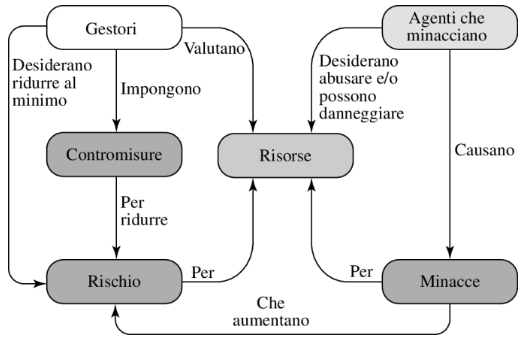
\includegraphics[width=0.95\linewidth]{chapters/images1/sicurezza.png}
    \caption{Concetti di sicurezza}
    \label{fig:sec}
\end{figure}

\begin{itemize}
    \item \textbf{Attacchi} alla sicurezza: qualsiasi azione che comprometta la sicurezza di un'informazione
    \item \textbf{Meccanismi} di sicurezza: un processo progettato per rilevare, prevenire o recuperare da un attacco
    \item \textbf{Servizi} di sicurezza: contrastano gli attacchi, si avvalgono di uno o più meccanismi per fornire il servizio
\end{itemize}

\subsubsection{Attacchi passivi e attivi}
\begin{itemize}
    \item \textbf{Attacchi passivi:} NON alterano le informazioni; lo scopo dell'attacco è ottenere informazioni sui messaggi trasmessi
    \begin{itemize}
        \item accesso al contenuto del messaggio
        \item analisi del traffico di rete (la frequenza o la lunghezza dei messaggi potrebbero rivelare la natura della comunicazione)
    \end{itemize}
    \item \textbf{Attacchi attivi:} modificano il flusso delle informazioni
    \begin{itemize}
        \item fingere di essere qualcun'altro
        \item denial of service
    \end{itemize}
\end{itemize}

\section{Minacce e conseguenze}
Per threat si intende una potenziale violazione della sicurezza.

Le azioni che potrebbero causare una violazione devono essere protette o preparate; queste azione vengono chiamate \textbf{attacchi}.

Le minacce possono essere divise in quattro gruppi:
\begin{itemize}
    \item \textbf{Divulgazione non autorizzata;} è una minaccia alla confidenzialità.
    \begin{itemize}
        \item \textbf{esposizione}: un errore umano, software o hardware conduce alla rivelazione di dati sensibili
        \item \textbf{intercettazione}
        \item \textbf{inferenza}: l'attaccante è in grado di ottenere dalla sola osservazione del traffico
        \item \textbf{intrusione}: un attaccante ottiene accesso a dati sensibili superando un controllo di accesso
    \end{itemize}
    \item \textbf{Inganno;} è una minaccia all'integrità dei dati.
    \begin{itemize}
        \item \textbf{mascheramento:} tentativo da parte dell'attacante di ottenere l'accesso a un sistema fingendosi un utente autorizzato
        \item \textbf{falsificazione:} alterazione di dati validi o inserimento di dati falsi in un database
        \item \textbf{ripudio:} un utente rinnega di aver inviato o ricevuto dei dati
    \end{itemize}
    \item \textbf{Interruzione;} è una minaccia alla disponibilità o integrità di un sistema
    \begin{itemize}
        \item \textbf{interdizione:} danneggiamento dell'hardware
        \item \textbf{corruzione:} le risorse funzionano in modo non voluto
        \item \textbf{ostruzione:} interferire con le comunicazioni alterandone i collegamenti
    \end{itemize}
    \item \textbf{Usurpazione;} è una minaccia all'integrità del sistema.
    \begin{itemize}
        \item \textbf{approprazione indebita:} ad esempio una sottrazione del servizio (DDOS)
        \item \textbf{uso improprio:} ad esempio dopo che un utente ha ottenuto un accesso non autorizzato  
    \end{itemize}
\end{itemize}

\section{Principi fondamentali di progettazione della sicurezza}

Sono delle regole generali della sicurezza informatica. 

\subsection{Principle of Fail-Safe Defaults (default libero da fallimento)}

A meno che un soggetto non abbia accesso esplicito a un oggetto, dovrebbe essergli negato l'accesso a tale oggetto.

In caso di fallimento del sistema, il sistema deve rimanere in uno stato di sicurezza

\subsection{Principle of Economy of Mechanism (economia dei meccanismi)}

I meccanismi di sicurezza dovrebbero essere il più semplice possibile; questo implica meno errori, meno controlli e testing; nella complessità si nasconde
 una maggiore possibilità di fallimenti o vulnerabilità.

\subsection{Principle of Complete Mediation}

Ogni accesso ad una risorsa deve sempre essere controllato da un meccanismo di sicurezza.


\subsection{Principle of Open Design}

La sicurezza di un meccanismo non dovrebbe dipendere dalla segretezza della sua progettazione
o attuazione.

La sicurezza non deve essere garantita dal fatto che l'attaccante non sa come è stata progettata una cosa.

\subsection{Principle of Separation of Privilege}

Un sistema non dovrebbe concedere l'autorizzazione in base a una singola condizione;
principio di separazione dei doveri.

\subsection{Principle of Least Privilege (privilegio minimo)}

A un soggetto dovrebbero essere concessi solo i privilegi di cui ha bisogno per completare il suo
compito.

Un caso di eccezione può essere quando per determinate azioni, il diritto di accesso del soggetto può essere
aumentato ma rilasciato immediatamente al completamento dell'azione.

\subsection{Principle of Psychological Acceptability}

I meccanismi di sicurezza non dovrebbero rendere l'accesso alla risorsa più difficile che se i
meccanismi di sicurezza non fossero presenti.

\section{Superificie di attacco}
È costituita dalle vulnerabilità raggiungibili e sfruttabili in un sistema, come ad esempio:
\begin{itemize}
    \item le porte aperte verso l'esterno
    \item servizi disponibili all'interno di un firewall
    \item codice che elabora dati in entrata
    \item un dipendente con accesso a dei dati sensibili (social engeneering)
\end{itemize}

Alcune superfici di attacco:
\begin{itemize}
    \item \textbf{superificie di attacco di rete}; sono incluse vulnerabilità del protocollo di rete
    \item \textbf{superificie di attacco software}; sono incluse vulnerabilità nel codice delle applicazioni
    \item \textbf{superificie di attacco umano;} sono incluse vulnerabilità create dal personale (errori, social engeneering)
\end{itemize}

\section{Progettazione della Sicurezza}

Una strategia di sicurezza globale comprende tre aspetti:
\begin{itemize}
    \item \textbf{Specifiche/Politiche:} cosa dovrebbe fare lo schema di sicurezza?
    \item \textbf{Implementazione/Meccanismi:} come funziona?
    \item \textbf{Correttezza/Sicurezza:} funziona davvero?
\end{itemize}

\subsection{Implementazione della Sicurezza}

Prevede quattro linee d'azione complementari:
\begin{itemize}
    \item \textbf{Prevenzione:} uno schema di sicurezza ideale è uno schema in cui nessun attacco ha successo
    \item \textbf{Detection (rilevamento):} ad esempio sistemi di rilevamento di instrusioni
    \item \textbf{Risposta:} se viene rilevato un attacco, rispondere in modo tale da fermarlo ed evitare ulteriori danni 
    \item \textbf{Recovery (ripristino):} ad esempio l'uso di sistemi di backup nel caso in cui venga compromessa l'integrità dei dati
\end{itemize}



